\section{Auswertung}
\label{sec:Auswertung}
Mittelwert der Federkonstanten $D = \frac{F}{\triangle x}$ für $n = 10$ Messdaten: 
\begin{equation}
\langle D \rangle = \frac{1}{n} \sum_i=1^n D_i = \SI{0.029}{\newton\per\centi\meter}
\end{equation}

\begin{figure}
    \centering
    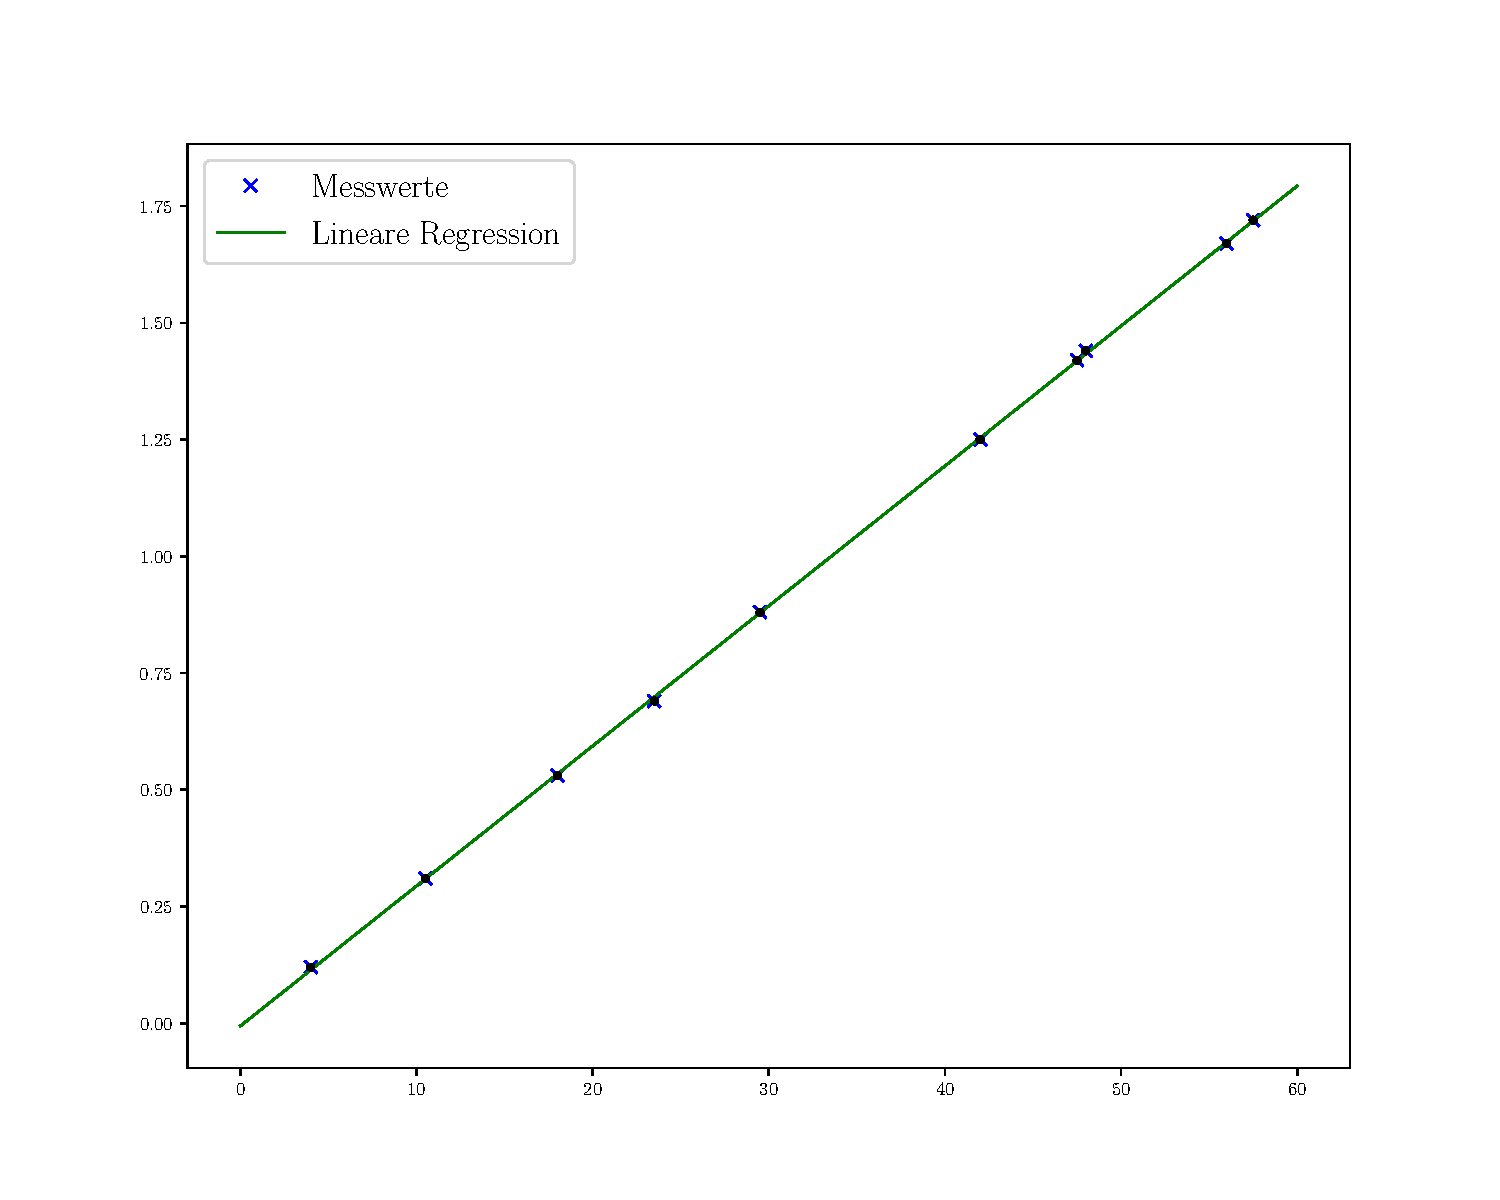
\includegraphics{Plot.pdf}
    \caption{Plot.}
    \label{fig:plot}
  \end{figure}
  
  
  Siehe \autoref{fig:plot}!